\documentclass[border=1cm]{standalone}
\usepackage{tikz}
\usepackage{amsmath,amssymb}
\usetikzlibrary{arrows.meta, decorations.markings, calc}

\begin{document}
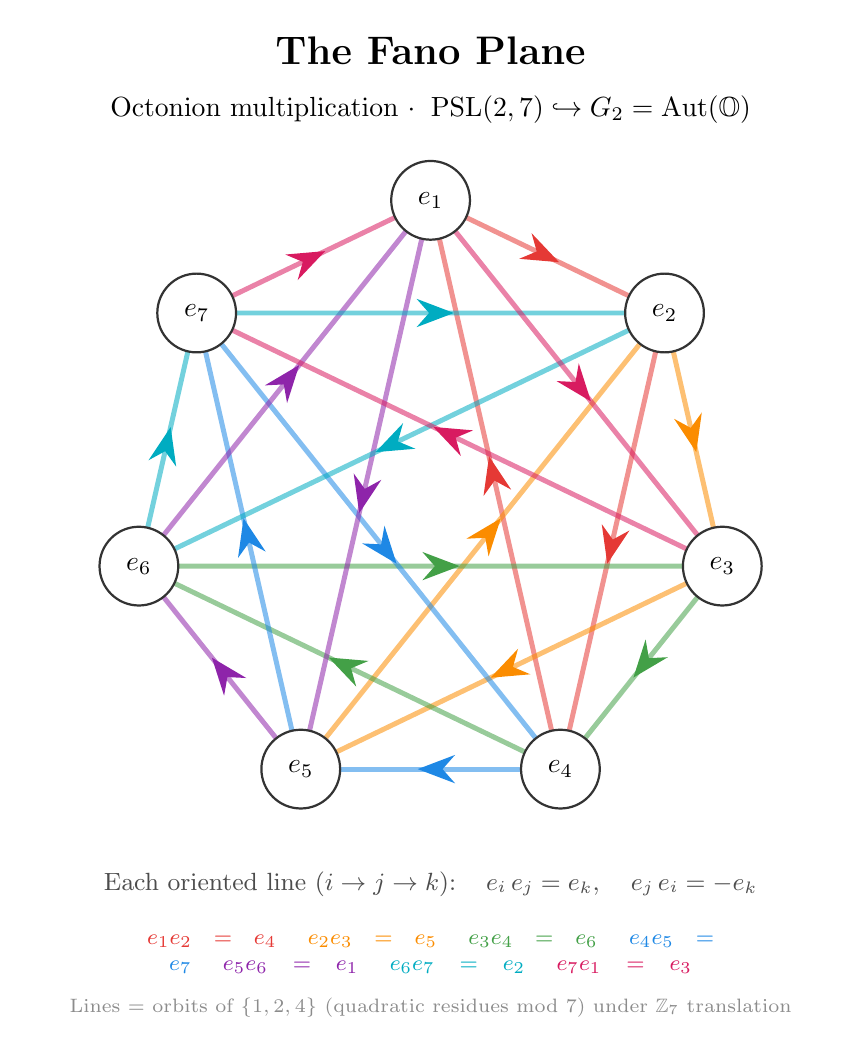
\begin{tikzpicture}[
    vertex/.style={circle, draw=black!80, fill=white, minimum size=10mm,
                   inner sep=0pt, font=\normalsize, line width=0.8pt},
    oriented line/.style={line width=1.8pt, opacity=0.55,
        decoration={markings,
            mark=at position 0.55 with {\arrow[scale=1.2, opacity=1]{Stealth}}},
        postaction={decorate}},
]

% Circle radius
\def\R{3.8}

% 7 vertices equally spaced, starting from top (vertex 1 at 90°)
\foreach \i in {1,...,7} {
    \pgfmathsetmacro{\angle}{90 - (\i-1)*360/7}
    \coordinate (P\i) at (\angle:\R);
}

% Colors for the 7 lines
\definecolor{c1}{HTML}{E53935}  % red
\definecolor{c2}{HTML}{FB8C00}  % orange
\definecolor{c3}{HTML}{43A047}  % green
\definecolor{c4}{HTML}{1E88E5}  % blue
\definecolor{c5}{HTML}{8E24AA}  % purple
\definecolor{c6}{HTML}{00ACC1}  % cyan
\definecolor{c7}{HTML}{D81B60}  % pink

% Draw the 7 Fano lines as oriented triangles
% Each line {a,b,c}: e_a * e_b = e_c (cyclic)
% Lines are orbits of {1,2,4} under +1 mod 7
%   {1,2,4}, {2,3,5}, {3,4,6}, {4,5,7}, {5,6,1}, {6,7,2}, {7,1,3}
% Oriented: (a → b → c → a) means e_a·e_b = e_c, e_b·e_c = e_a, e_c·e_a = e_b

% Draw oriented edges for each line (3 directed edges per line = oriented triangle)
\foreach \a/\b/\c/\col in {1/2/4/c1, 2/3/5/c2, 3/4/6/c3, 4/5/7/c4, 5/6/1/c5, 6/7/2/c6, 7/1/3/c7} {
    \draw[\col, oriented line] (P\a) -- (P\b);
    \draw[\col, oriented line] (P\b) -- (P\c);
    \draw[\col, oriented line] (P\c) -- (P\a);
}

% Draw vertices on top
\foreach \i in {1,...,7} {
    \pgfmathsetmacro{\angle}{90 - (\i-1)*360/7}
    % Subtle colored ring based on which lines pass through this vertex
    \node[vertex] at (\angle:\R) {$e_{\i}$};
}

% Title
\node[above, font=\Large\bfseries] at (0, \R + 1.6) {The Fano Plane};
\node[above, font=\normalsize] at (0, \R + 0.85) {%
    Octonion multiplication $\cdot\;\; \mathrm{PSL}(2,7) \hookrightarrow G_2 = \mathrm{Aut}(\mathbb{O})$};

% Subtitle: the rule
\node[below, font=\small, text=black!70] at (0, -\R - 0.8) {%
    Each oriented line $(i \to j \to k)$: \;
    $e_i \, e_j = e_k$, \;\;
    $e_j \, e_i = -e_k$};

% The multiplication table at bottom
\node[below, font=\footnotesize, text=black!60, text width=10cm, align=center] at (0, -\R - 1.6) {%
    \textcolor{c1}{$e_1 e_2 = e_4$} \quad
    \textcolor{c2}{$e_2 e_3 = e_5$} \quad
    \textcolor{c3}{$e_3 e_4 = e_6$} \quad
    \textcolor{c4}{$e_4 e_5 = e_7$} \quad
    \textcolor{c5}{$e_5 e_6 = e_1$} \quad
    \textcolor{c6}{$e_6 e_7 = e_2$} \quad
    \textcolor{c7}{$e_7 e_1 = e_3$}};

% Bottom note
\node[below, font=\scriptsize, text=black!45] at (0, -\R - 2.4) {%
    Lines = orbits of $\{1,2,4\}$ (quadratic residues mod $7$) under $\mathbb{Z}_7$ translation};

\end{tikzpicture}
\end{document}
